\documentclass[12pt]{article}
\usepackage{graphicx}
\usepackage[a4paper, margin=1in]{geometry}
\usepackage{amsmath}
\usepackage[utf8]{inputenc}
\usepackage{listings}
\usepackage{xcolor}

\usepackage{amsfonts}
\usepackage{amssymb}
\usepackage{geometry}
\usepackage{titlesec}
\usepackage{fancyhdr}
\usepackage{lipsum}


\lstdefinestyle{mystyle}{
    backgroundcolor=\color{white},
    commentstyle=\color{codegreen},
    keywordstyle=\color{magenta},
    numberstyle=\tiny\color{codegray},
    stringstyle=\color{codepurple},
    basicstyle=\ttfamily\footnotesize,
    breakatwhitespace=false,
    breaklines=true,
    captionpos=b,
    keepspaces=true,
    numbers=left,
    numbersep=5pt,
    showspaces=false,
    showstringspaces=false,
    showtabs=false,
    tabsize=2
}

\lstset{style=mystyle}

\definecolor{codegreen}{rgb}{0,0.6,0}
\definecolor{codegray}{rgb}{0.5,0.5,0.5}
\definecolor{codepurple}{rgb}{0.58,0,0.82}

% Configuración de página
\geometry{a4paper, margin=1in}
\pagestyle{fancy}
\fancyhf{}
\rhead{Eidan Owen Plata Salinas}
\lhead{CARACTERISTICAS FUNDAMENTALES}
\cfoot{\thepage}

% Títulos
\titleformat{\section}[block]{\normalfont\Large\bfseries}{\thesection}{1em}{}
\titlespacing*{\section}{0pt}{\baselineskip}{\baselineskip}



\title{CARACTERISTICAS FUNDAMENTALES: ALGORITMO GENETICO VS PCA}
\author{Plata Salinas Eidan Owen}
\date{\today}

\begin{document}
\maketitle
\pagebreak

\section*{Introducción}
La elección de las características fundamentales de un dataset es un aspecto crítico en la investigación y análisis de datos en la actualidad. La calidad de los resultados y las conclusiones obtenidas de cualquier estudio depende en gran medida de la selección adecuada de las variables o características que se incluyen en el conjunto de datos. Esta etapa inicial de la investigación de datos es fundamental, ya que determina en gran medida la eficacia de los algoritmos de análisis y las predicciones que se pueden obtener posteriormente [1]. \vspace{1cm}

La importancia de la selección de características radica en varios aspectos clave. En primer lugar, una selección cuidadosa de características puede ayudar a reducir la dimensionalidad de un conjunto de datos, lo que a su vez mejora la eficiencia computacional y evita problemas como la maldición de la dimensionalidad. Además, al elegir las características adecuadas, se pueden eliminar variables irrelevantes o ruidosas que podrían introducir sesgos o distorsiones en el análisis. Esto conduce a modelos más precisos y resultados más confiables [2]. \vspace{1cm}

Existen numerosos métodos y enfoques para la selección de características, que van desde técnicas estadísticas hasta algoritmos de aprendizaje automático. Algunos de los métodos más comunes incluyen el análisis de componentes principales (PCA), la eliminación de características con baja varianza, la selección basada en la importancia de características, y enfoques de búsqueda exhaustiva o heurística. La elección del método adecuado depende en gran medida del tipo de datos, el objetivo del estudio y las limitaciones computacionales [3]. \vspace{1cm}

La elección de las características fundamentales de un dataset es un proceso crucial en la investigación de datos. Requiere un enfoque estratégico y un profundo conocimiento del dominio del problema. La selección cuidadosa de características puede mejorar la calidad de los resultados, reducir la complejidad computacional y aumentar la interpretabilidad de los modelos. Sin embargo, es importante recordar que la selección de características es solo una parte del proceso de análisis de datos, y su eficacia depende de la atención continua a otros aspectos como la limpieza de datos, la ingeniería de características y la validación de modelos. En última instancia, una elección inteligente de características allana el camino hacia la obtención de conocimientos valiosos a partir de los datos [4]. \vspace{1cm}

El Análisis de Componentes Principales (PCA) es un poderoso algoritmo de reducción de dimensionalidad ampliamente utilizado en el campo del análisis de datos y la estadística. Su objetivo principal es transformar un conjunto de datos original en un nuevo conjunto de datos, donde las variables originales se reemplazan por un conjunto más pequeño de variables llamadas componentes principales. Estos componentes principales son combinaciones lineales de las variables originales y están diseñados para capturar la mayor variabilidad posible en los datos. PCA es especialmente útil cuando se trabaja con conjuntos de datos de alta dimensionalidad, ya que puede ayudar a reducir la complejidad y a eliminar la multicolinealidad entre las variables. Además de la reducción de dimensionalidad, PCA también se utiliza en aplicaciones como la visualización de datos, la compresión de imágenes y la eliminación de ruido en señales, lo que lo convierte en una herramienta versátil en el análisis de datos y la minería de datos [5]. \vspace{1cm}

Los Algoritmos Genéticos (AG) son una familia de técnicas de optimización que pueden utilizarse para abordar la selección de características de manera más directa. Los AG trabajan con un conjunto inicial de características, evalúan diferentes subconjuntos de características en función de un criterio de aptitud y evolucionan hacia subconjuntos óptimos a través de generaciones de selección, cruzamiento y mutación. Esta capacidad para explorar exhaustivamente el espacio de características puede ser especialmente útil cuando se enfrenta a conjuntos de datos complejos y no lineales, y cuando se busca una selección de características más precisa y específica para una tarea en particular [6]. \vspace{1cm}

En última instancia, la elección entre PCA y Algoritmos Genéticos en la selección de características depende de las características del problema y de los objetivos del análisis. PCA es útil para reducir la dimensionalidad y mantener la estructura global de los datos, pero puede no ser adecuado cuando se requiere una selección de características más precisa. Los Algoritmos Genéticos, por otro lado, ofrecen un enfoque más flexible y personalizable para la selección de características, pero pueden requerir más recursos computacionales y ajuste de parámetros. En muchos casos, una combinación de ambos enfoques o el uso de otros métodos de selección de características específicos del dominio pueden ser la mejor estrategia. La elección adecuada debe basarse en una comprensión profunda del problema y las características del conjunto de datos en cuestión [7]. \vspace{1cm}
\clearpage

\section*{Desarrollo}

\subsection*{FUNCION CARGAR DATOS}

Utiliza pd.read\_csv para leer el archivo CSV especificado en ruta\_csv. La opción header=None indica que el archivo no tiene fila de encabezado. X es asignado a todas las columnas excepto la última, que se supone contienen las características (features) de los datos. es asignado a la última columna, que se supone es la variable objetivo (target). Retorna X (características) Y y (objetivo).\vspace{1cm}

\begin{lstlisting}[language=Python]
def cargar_datos(ruta_csv):
	data = pd.read_csv(ruta_csv, header=None)
	X = data.iloc[:, :-1].values
	y = data.iloc[:, -1].values
	return X, y
\end{lstlisting}


\subsection*{FUNCION K FOLD CROSS VALIDATION}

Utiliza StratifiedKFold para dividir los datos en k conjuntos, manteniendo la proporción de las clases en cada partición. Itera sobre los conjuntos de entrenamiento y prueba generados, entrenando y evaluando el modelo en cada iteración. Clona el modelo para cada iteración usando clone(modelo) para asegurar que cada evaluación es independiente. Calcula y guarda la precisión (accuracy) del modelo en cada iteración. Retorna una lista de las puntuaciones de precisión obtenidas. \vspace{1cm}

\begin{lstlisting}[language=Python]
def k_fold_cross_validation(X, y, k, modelo):
	skf = StratifiedKFold(n_splits=k, shuffle=True, random_state=42)
	scores = []
	
	for train_index, test_index in skf.split(X, y):
		X_train, X_test = X[train_index], X[test_index]
		y_train, y_test = y[train_index], y[test_index]
		
		modelo_clonado = clone(modelo)
		modelo_clonado.fit(X_train, y_train)
		
		y_pred = modelo_clonado.predict(X_test)
		score = accuracy_score(y_test, y_pred)
		scores.append(score)
	
	return scores
\end{lstlisting}


\subsection*{FUNCION GENERAR POBLACION INICIAL}

Crea una matriz binaria aleatoria de tamaño tam\_poblacion x num\_caracteristicas. Cada fila de la matriz representa un ``individuo'' en la población, con cada columna representando la presencia o ausencia de una característica (1 o 0). Retorna esta matriz poblacional. \vspace{1cm}

\begin{lstlisting}[language=Python]
def generar_poblacion_inicial(num_caracteristicas, tam_poblacion=10):
	return np.random.randint(2, size=(tam_poblacion, num_caracteristicas))
\end{lstlisting}

\subsection*{FUNCION REPRODUCIR}

Para cada nueva generación, selecciona al azar dos padres de la población existente. Genera dos hijos por cada par de padres, dividiendo y combinando sus "genes" (características) en un punto aleatorio. Repite este proceso hasta crear una nueva población de tamaño igual al doble de los individuos originales.
Retorna la nueva población. \vspace{1cm}

\begin{lstlisting}[language=Python]
	def reproducir(individuos):
		nuevos_individuos = []
		for _ in range(10): 
			padres = np.random.choice(len(individuos), 2, replace=False)
			punto_cruce = np.random.randint(1, len(individuos[0]))
			hijo1 = np.concatenate([individuos[padres[0]][:punto_cruce], individuos[padres[1]][punto_cruce:]])
			hijo2 = np.concatenate([individuos[padres[1]][:punto_cruce], individuos[padres[0]][punto_cruce:]])
			nuevos_individuos.extend([hijo1, hijo2])
		return nuevos_individuos
\end{lstlisting}


\subsection*{FUNCION MUTAR}

Itera sobre cada individuo y cada gen (característica) del individuo. Con una probabilidad prob\_mutacion, cambia el gen (de 0 a 1 o de 1 a 0). Esto introduce variabilidad en la población, lo cual es clave en los algoritmos genéticos. Retorna la población mutada. \vspace{1cm}

\begin{lstlisting}[language=Python]
def mutar(individuos, prob_mutacion=0.1):
	for individuo in individuos:
		for i in range(len(individuo)):
			if np.random.rand() < prob_mutacion:
			individuo[i] = 1 - individuo[i]
	return individuos
\end{lstlisting}


\subsection*{FUNCION EVALUAR INDIVIDUOS}

Itera sobre cada individuo de la población. Si un individuo no tiene características seleccionadas (suma igual a 0), su puntuación es 0. Para los demás, selecciona las características correspondientes del conjunto de datos X basándose en los genes (1 o 0) del individuo. Crea un pipeline con escalado estándar y el modelo de clasificación proporcionado. Aplica validación cruzada k-fold al conjunto de datos filtrado y calcula la precisión media. Retorna una lista de puntuaciones, una para cada individuo. \vspace{1cm}

\begin{lstlisting}[language=Python]

def evaluar_individuos(X, y, individuos, k=5, modelo=LogisticRegression()):
	puntuaciones = []
	for individuo in individuos:
		if np.sum(individuo) == 0:
			puntuaciones.append(0)
			continue
	
		caracteristicas_seleccionadas = X[:, individuo.astype(bool)]
		pipeline = Pipeline([('scaler', StandardScaler()), ('classifier', modelo)])
		scores = k_fold_cross_validation(caracteristicas_seleccionadas, y, k, pipeline)
		puntuaciones.append(np.mean(scores))
	return puntuaciones

\end{lstlisting}


\subsection*{FUNCION SELECCIONAR MEJORES}

Ordena a los individuos según sus puntuaciones. Selecciona el número especificado de los mejores individuos (los que tienen las puntuaciones más altas). Retorna estos individuos seleccionados. \vspace{1cm}

\begin{lstlisting}[language=Python]
	
def seleccionar_mejores(individuos, puntuaciones, num_seleccionados=10):
	indices = np.argsort(puntuaciones)[-num_seleccionados:]
	return [individuos[i] for i in indices]
	
\end{lstlisting}


\subsection*{FUNCION COMPARAR MODELOS}

Entrena y evalúa el modelo proporcionado primero con todas las características (X completo) y luego solo con las características importantes. Utiliza validación cruzada k-fold en ambos casos. Imprime las precisiones medias para cada caso, proporcionando una comparación directa. \vspace{1cm}

\begin{lstlisting}[language=Python]
	
def comparar_modelos(X, y, caracteristicas_importantes, modelo=LogisticRegression()):
	pipeline_completo = Pipeline([('scaler', StandardScaler()), ('classifier', modelo)])
	scores_completo = k_fold_cross_validation(X, y, 5, pipeline_completo)
	
	X_reducido = X[:, caracteristicas_importantes]
	pipeline_reducido = Pipeline([('scaler', StandardScaler()), ('classifier', modelo)])
	scores_reducido = k_fold_cross_validation(X_reducido, y, 5, pipeline_reducido)
	
	print(f"Efectividad promedio usando todas las caracteristicas: {np.mean(scores_completo):.2f}")
	print(f"Efectividad promedio usando caracteristicas seleccionadas: {np.mean(scores_reducido):.2f}")
	
\end{lstlisting}

\subsection*{FUNCION APLICAR PCA Y COMPARAR}

Reduce la dimensionalidad de X a num\_componentes utilizando PCA. Entrena y evalúa el modelo de clasificación proporcionado en el conjunto de datos transformado. Utiliza validación cruzada k-fold y calcula la precisión media. Imprime la precisión media y retorna las puntuaciones obtenidas. \vspace{1cm}

\begin{lstlisting}[language=Python]
	
def aplicar_pca_y_comparar(X, y, num_componentes, modelo=LogisticRegression()):
	pca = PCA(n_components=num_componentes)
	X_pca = pca.fit_transform(X)
	
	pipeline_pca = Pipeline([('scaler', StandardScaler()), ('classifier', modelo)])
	scores_pca = k_fold_cross_validation(X_pca, y, 5, pipeline_pca)
	
	print(f"Efectividad promedio usando PCA con {num_componentes} componentes: {np.mean(scores_pca):.2f}")
	
	return scores_pca
	
\end{lstlisting}


\subsection*{FUNCION MAIN}

Carga los datos y genera una población inicial para el algoritmo genético. Ejecuta el algoritmo genético para varias generaciones, reproduciendo, mutando y seleccionando los mejores individuos. Al final, identifica las características importantes, compara los modelos con y sin estas características y aplica PCA para una comparación adicional. Finalmente, imprime los resultados relevantes. \vspace{1cm}

\begin{lstlisting}[language=Python]
	
def main(ruta_csv, num_generaciones=10, num_componentes_pca=4):
	X, y = cargar_datos(ruta_csv)
	num_caracteristicas = X.shape[1]
	poblacion = generar_poblacion_inicial(num_caracteristicas)
	
	for _ in range(num_generaciones):
		descendientes = reproducir(poblacion)
		descendientes_mutados = mutar(descendientes)
		copia_poblacion = mutar(poblacion.copy())
		poblacion_total = np.vstack((poblacion, copia_poblacion, descendientes_mutados))
		puntuaciones = evaluar_individuos(X, y, poblacion_total)
		poblacion = seleccionar_mejores(poblacion_total, puntuaciones)
	
	mejor_individuo = poblacion[0]
	caracteristicas_importantes = np.where(mejor_individuo == 1)[0]
	print("CaracterIsticas importantes:", caracteristicas_importantes)
	
	comparar_modelos(X, y, caracteristicas_importantes)
	scores_pca = aplicar_pca_y_comparar(X, y, num_componentes_pca)
	
\end{lstlisting}

\subsection*{Resultados}

\begin{figure}[h]
	\centering % para centrar la imagen
	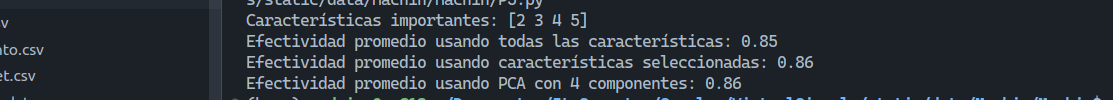
\includegraphics[width=1\textwidth]{krn} % Cambia 'ruta/al/archivo.jpg' por la ruta de tu imagen
	\caption{Resultados de la ejecución} % El texto del pie de imagen
	\label{fig:imagen1} % Etiqueta para referenciar la imagen
\end{figure}


\clearpage




\subsection*{Referencias}


[1] Diccionario. “Dataset: Qué es y principales características”. The Data Schools. Accedido el 22 de noviembre de 2023. [En línea]. Disponible: https://thedataschools.com/que-es/data-set/\vspace{1cm}

[2] Blog Tecnico. “Algoritmo PCA: De lo mucho a lo poco | LIS Data Solutions”. LIS Data Solutions. Accedido el 22 de noviembre de 2023. [En línea]. Disponible: https://www.lisdatasolutions.com/es/blog/algoritmo-pca-de-lo-mucho-a-lo-poco/\vspace{1cm}

[3] Amazon Web Services. “Algoritmo de analisis de componente principal (PCA) - Amazon SageMaker”. Accedido el 22 de noviembre de 2023. [En línea]. Disponible: https://docs.aws.amazon.com/es\_es/sagemaker/latest/dg/pca.html\vspace{1cm}

[4] J. Alquicira. “Análisis de componentes principales (PCA)”. Conogasi. Accedido el 22 de noviembre de 2023. [En línea]. Disponible: https://conogasi.org/articulos/analisis-de-componentes-principales-pca/\vspace{1cm}

[5] SITIOBIGDATA. “Interpretar dataset en machine learning - sitiobigdata.com”. sitiobigdata.com. Accedido el 22 de noviembre de 2023. [En línea]. Disponible: https://sitiobigdata.com/2018/08/27/interpretar-dataset-en-machine-learning/\vspace{1cm}

[6] Microsoft. “DataSets - ADO.NET”. Microsoft Learn: Build skills that open doors in your career. Accedido el 22 de noviembre de 2023. [En línea]. Disponible: https://learn.microsoft.com/es-es/dotnet/framework/data/adonet/ado-net-datasets\vspace{1cm}

[7] Conogasi. “Algoritmos genéticos”. Conogasi. Accedido el 22 de noviembre de 2023. [En línea]. Disponible: https://conogasi.org/articulos/algoritmos-geneticos/\vspace{1cm}


\clearpage

\vspace{1cm}\vspace{1cm}


\section{Còdigo completo}

\begin{lstlisting}[language=Python]

import csv
import pandas as pd
from sklearn.model_selection import train_test_split
import numpy as np

class CascadeSVM:
def __init__(self, learning_rate=0.01, n_iterations=1000, lambda_param=0.1):
self.clf_dh = LinearSVM(learning_rate=learning_rate, n_iterations=n_iterations, lambda_param=lambda_param)
self.clf_sl = LinearSVM(learning_rate=learning_rate, n_iterations=n_iterations, lambda_param=lambda_param)

def print_weights(self):
print("Weights for DH Classifier:")
print("------------------------------")
for idx, w in enumerate(self.clf_dh.weights):
print(f"Feature {idx+1}: {w:.5f}")
print(f"Bias (DH Classifier): {self.clf_dh.bias:.5f}\n")

print("Weights for SL Classifier:")
print("------------------------------")
for idx, w in enumerate(self.clf_sl.weights):
print(f"Feature {idx+1}: {w:.5f}")
print(f"Bias (SL Classifier): {self.clf_sl.bias:.5f}")

def fit(self, X, y):
y_dh = np.where(y == 'DH', 1, -1)
self.clf_dh.fit(X, y_dh)

mask = y != 'DH'
X_sl = X[mask]
y_sl = np.where(y[mask] == 'SL', 1, -1)
self.clf_sl.fit(X_sl, y_sl)

def predict(self, X):
preds = []

dh_predictions = self.clf_dh.predict(X)
sl_predictions = self.clf_sl.predict(X)

for idx, (dh_pred, sl_pred) in enumerate(zip(dh_predictions, sl_predictions)):
if dh_pred == 1:
label = 'DH'
elif sl_pred == 1:
label = 'SL'
else:
label = 'NO'
preds.append(label)
print(f"Data {idx+1}: {X.iloc[idx].values} -> Predicted label: {label}")

return np.array(preds)

class LinearSVM:
def __init__(self, learning_rate=0.001, n_iterations=1000, lambda_param=0.1):
self.learning_rate = learning_rate
self.n_iterations = n_iterations
self.lambda_param = lambda_param
self.weights = None
self.bias = None

def fit(self, X, y):
n_samples, n_features = X.shape
self.weights = np.zeros(n_features)
self.bias = 0

for _ in range(self.n_iterations):
for idx, x_i in enumerate(X.values):
condition = y[idx] * (np.dot(x_i, self.weights) - self.bias) >= 1
if condition:
dw = 2 * self.lambda_param * self.weights
db = 0
else:
dw = 2 * self.lambda_param * self.weights - np.dot(x_i, y[idx])
db = y[idx]
self.weights -= self.learning_rate * dw
self.bias -= self.learning_rate * db

def predict(self, X):
linear_output = np.dot(X, self.weights) - self.bias
return np.sign(linear_output)

def dat_to_csv(dat_filename, csv_filename):
with open(dat_filename, 'r') as dat_file:
lines = dat_file.readlines()
with open(csv_filename, 'w', newline='') as csv_file:
writer = csv.writer(csv_file, delimiter=',')
for line in lines:
data = line.split()[:]
writer.writerow(data)

def csv_datos(nombre_archivo):
datos = []
with open(nombre_archivo, newline='') as archivo_csv:
lector_csv = csv.reader(archivo_csv, delimiter=',')
for fila in lector_csv:
datos.append(','.join(fila))

csv_data = '\n'.join(datos)
return csv_data

def process_csv(data: str):
from io import StringIO
data_io = StringIO(data)
df = pd.read_csv(data_io, header=None)
X = df.iloc[:, :-1]
y = df.iloc[:, -1]
X_train, X_test, y_train, y_test = train_test_split(X, y, test_size=0.2, random_state=42)

return X_train, X_test, y_train, y_test

dat_filename = 'datata.dat'
csv_filename = 'dataset.csv'
dat_to_csv(dat_filename, csv_filename)
X_train, X_test, y_train, y_test = process_csv(csv_datos('dataset.csv'))
clf_cascade = CascadeSVM(learning_rate=0.01, n_iterations=1000, lambda_param=0.1)
clf_cascade.fit(X_train, y_train)
clf_cascade.print_weights()
y_pred = clf_cascade.predict(X_test)
accuracy = np.mean(y_pred == y_test)
print(f"Accuracy: {accuracy * 100:.2f}%")


\end{lstlisting}

\clearpage


\end{document}
